% !TEX root = ../thesis.tex
\section{Analýza dat a první modely}
\label{chap:experiments:analysis}

Rozpoznávání řeči se věnuje nemalé usílí již od 50. let 2O. století a v současné době nikoho nepřekvapí téměř bezchybně fungující obecný rozpoznávač v mobilních zařízeních. Pro obecné systémy dokonce existují korpusy s desítkami či stovkami a více hodin promluv, které je možné využít při vytváření těchto systémů.

Tyto korpusy však obsahují ve většině případů pouze \uv{standardní}\footnote{Slovením spojením \uv{standardní řeč} je myšlena řeč neobsahující vyrazné řečové vady, případně jiné formy produkce a často v nepřílíš akusticky náročném prostředí.} řeč. Pokud je snaha vytvořit nebo ověřit funkčnost systému za specifických podmínek (ať už se jedná o rušné prostředí či speciální typy promluv), tak je nezbytné získat potřebná data.

\subsection{Vytvoření korpusu EL promluv}

Na začátku byla idea o pomoci skupině lidí mající problémy s přirozenou řečí. Vůbec prvním předpokladem, na cestě k úspěšnému dosažení vůbec nějakého cíle, jsou data. Jelikož se jedná o velmi spefická data, tak je potřeba zajistit co možná největší množství kvalitních\footnote{Kvalitou je myšlena věrnost dat dané doméně, dále se mluví o přesnosti ve smyslu bezchybnosti přepisů.} a přesných dat.

V části \ref{sec:cause:desease} bylo zmíněno, že ročně se objevý více než 100 nových případů trvalé ztrázy hlasu ročně. Zaroveň bylo řečeno \cite{Skvrnakova2010}, že více rizikovými osobami jsou starší lidé, kteří intenzivně kouří a konzumují alkohol. Přesto je patrný trend snižujícího se věku pacientů a s tím souvisejícím nárůstem případů ztráty hlasu. Přičteme-li již zmíněný psychologický aspekt jeho ztráty, tak je zřejmé, jak komplikované je získat ke spolupráci i jen jednoho řečníka ochotného podstoupit naročné\footnote{I pro zdravého člověka je někdy někalikahodinové nahrávání vysilující. Pro jedince po TL to je z mnoha důvodů ještě řádově náročnější.} nahrávání.

Při libovolné práci s pacienty po TL, dřív nebo později dojde k určité formě spolupráce s oddělením ORL, které má nastarosti péči o tyto pacienty. V našem připadě nejprve s ORL klinikou při Fakultní nemocnici v Plzni a poté i s ORL klinikou Fakultní nemocnice v Motole. S jejich pomocí jsme získali ke spolupráci jednoho řečníka. Konkrétně se jedná o dámu v duchodovém věku, která podstoupila TL před více než 15 lety. Po překonání ostychu\footnote{Podle jejích vlastních slov nebyla schopna několik let po operaci ani zvednout nečekaný telefonní hovor, natož mluvit na veřejnosti.} se byla schopna naplno vrátit do běžného života a dokonce v určité formě opět přednášet o stomatologii na Lekařské fakultě v Plzni Univerzity Karlovy.

S její pomocí jsem, v 1. etapě nahrávání, byli schopni pořídit přes 10 hodin promluv, viz tabulka \ref{tab:experiments:analysis:recording}. Nahrávání probíhala v relativně spartánských podmínkách za plného běžného provozu katedry. Přesto získaná data neosahují žádný nežadoucí ruch, kromě toho produkovaného samotným EL.

Nahravací aparatůra sestávala z profesionálního mikrofonu (\todo{typ mikrofonu}{TBD}), předzesilovačem (TBD), externí zvukovou kartou a běžného notebooku. Mikrofon byl pomocí bezpolštářkové náplasti přilepen poblíž pravého koutku úst, abychom zaznamenaná řeč měla co možná nejvyšší kvalitu.

Celé nahrávání bylo v 1. etapě rozděleno do 14 samostatných sezení a probíhalo od prosince roku 2010 do května roku 2011. Každé sezení trvalo přibližně dvě hodiny během kterých se podařilo získat necelou hodinu akustických dat. Samotné nahrávání se sestávalo z 10 - 20 minutového úseku pořizování nahrávky a přibližně 10 minut dlouhého odpočinku. Ten byl nezbytný hlavně z důvodu únavy řečníka.

Ještě před samotným nahrávánám byly pečlivě vybrány a vytvořeny 2 sady vět:

\begin{enumerate}
  \item sada obsahující všechny možné české fonémy - \textit{40 vět}.
  \item sada obsahující věty s reálnou četností fonémů - \textit{5000 vět}.
\end{enumerate}

\noindent Pořízené nahrávky vždy odpovídají 10 - 20 minutovému úseku nepřerušovaného nahrávání a soubory tak vždy obsahují několik vět. Ty jsou od sebe odděleny minimálně 5 sekundovým úsekem ticha. Nahrávky dále mouhou obsahovat opakování chybně vyslovené věty, přeřeknutí, kýchnutí a další neřečové události. Z tohoto důvodu bylo nezbytné pořízené nahrávky anotovat, přestože byly pořízené na základě připravené sady vět.

Ještě před samotným anotováním byly nahrávky, podle úseků s tichem, rozsekány na menší části. V tomto případě úplně dobře nefungovali\footnote{Problémem byl zvuk EL, se kterým nebylo při návrhu VAD počítáno.} standardně používané sofistikovanější metody pro voice activity detection (angl. zkratka VAD), a proto bylo využito principu energie. Pro každou nahrávku obsahující více vět se pomocí vzorce

\begin{equation}
  \label{eq:experiments:analysis:energy}
  E_{RMS}(n) = \sqrt{\frac{1}{N} \sum_{n=1}^{N} \left| x(n) \right|^2},
\end{equation}

\noindent kde $N$ představuje počet vzorků v nahrávce a $x(n)$ představuje pravoúhlé okénko vzorku $n$. Pro tento případ se ukázalo jako vhodnější volit root-mean-square energy ($E_{RMS}$) a empericky se ukázalo, že vhodná délka okénka je v rozmezí $10 - 100$ ms. Na obrázku \ref{fig:experiments:analysis:speech} je zobrazena podoba audio signálu a spektrogram promluvy \textit{\uv{Akcie Komerční banky}}. Zároveň je zde vypočtené hodnoty energie a celková průměrná energie. Tyto hodntoty slouží pro určení míst kde začíná a končí věta. Na začátku a konci každé věty je dobré mít minimálně $0.5$ s ticha. Tím pádem, pokud energie nějakého úseku $x$ je $E_{RMS}(x) < avg(E_{RMS})$ a zároveň délka tohoto úseku $dur(x) \geq 1\ [s]$, tak nahrávku můžeme v tomto úseku rozdělit.

\begin{figure}[hbpt]
  \centering
  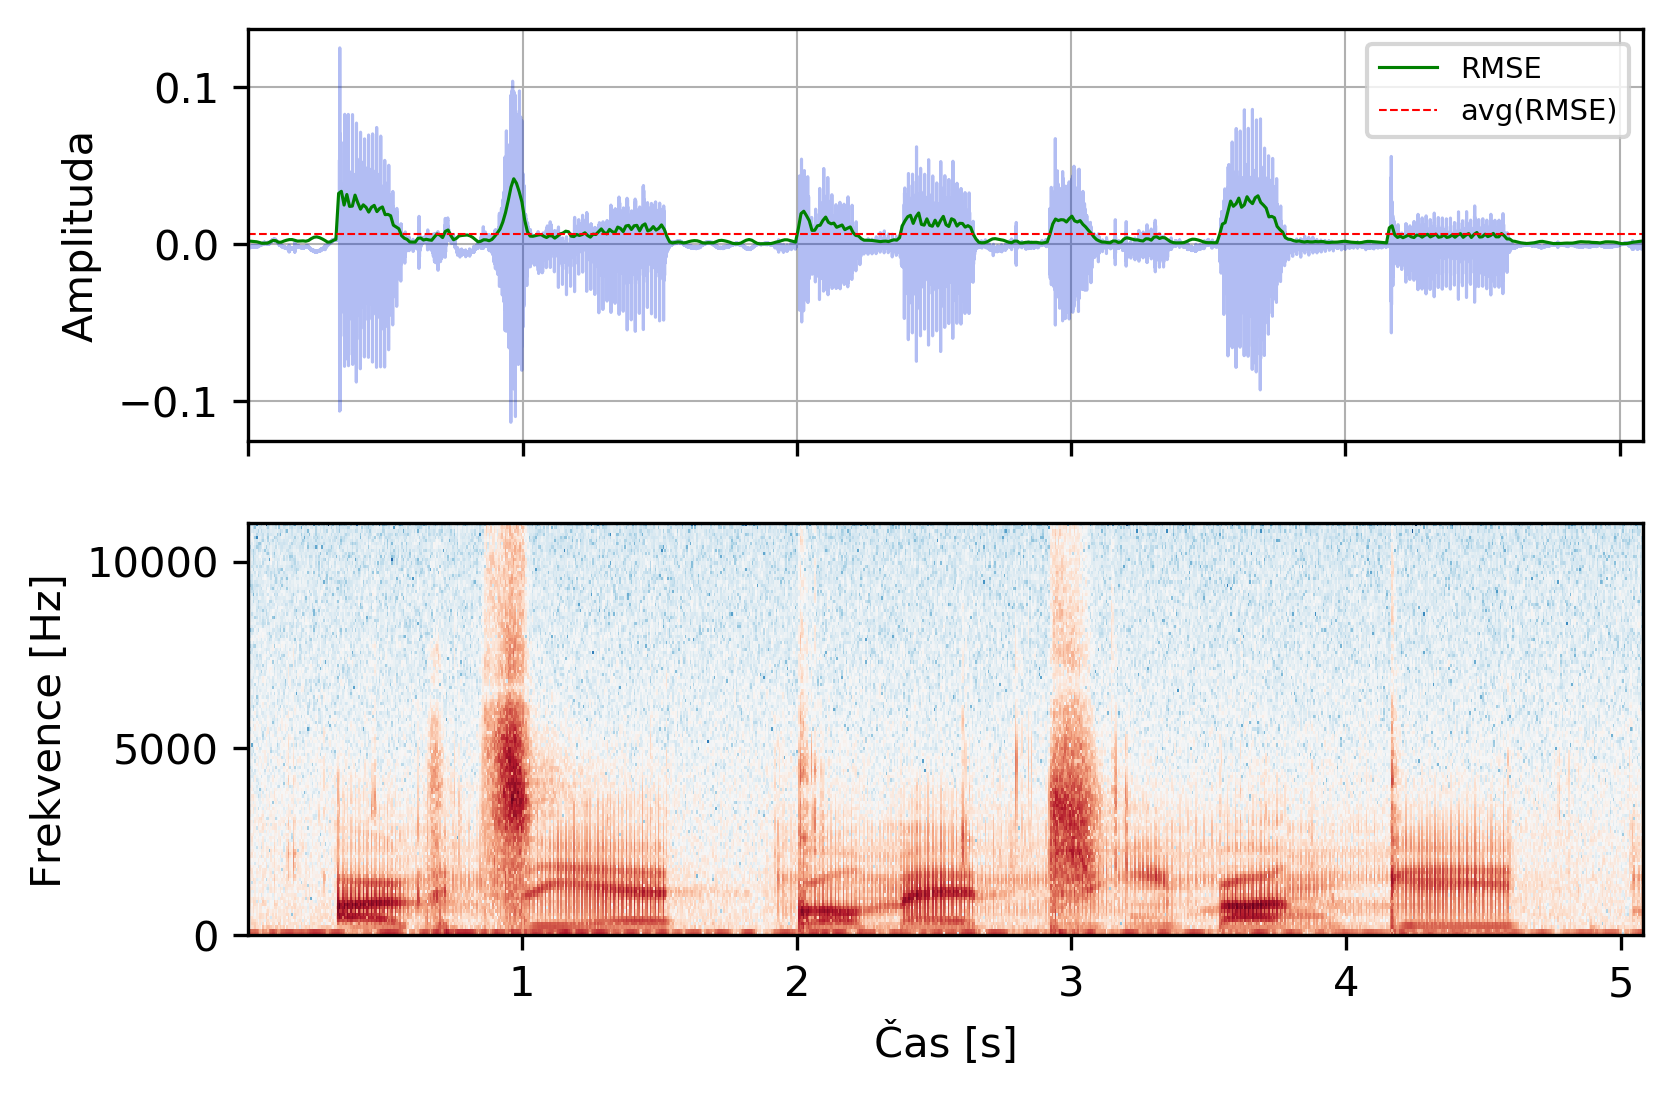
\includegraphics[width=0.8\textwidth]{./ch4-experiments/img/el_energy_spec.png}
  \caption{Průběh a spektrogram promluvy a vyznačenou energií promluvy.}
  \label{fig:experiments:analysis:speech}
\end{figure}

Samozřejmě pokud řečník v průbehu věty z libovolného důvodu udělal větší pauzu než $1$ s, tak tato věta byla rozdělena. Jelikož jsou výsledné kratší useky promluv následně anotovány, tak to nepředstavuje problém. Pro budoucí zpracování není podstatné zda promluva je opravdu celá věta, ale to jestli je tento úsek správně přepsán. Fakt, že některé věty jsou rozděleny je důvodem proč v tabulce \ref{tab:experiments:analysis:recording} více souborů než vět.

K anotaci posloužil interní nástroj určený k tomuto účelu a podíleli se na něm celkem 3 anotátoři z řad studentů, kteří si vzájemně kontrolovali své anotace. Ačkoli bylo potřeba anotovat relativně malé množství dat (cca 10 hodin audio záznamu), tak anotace zabrala přibližně 2 měsice. Hlavním důvodem byla relativně dlouhá doba, po kterou se anotátoři adaptovali na specificka EL řeči. Problémem bylo to, že nejprve nebyli vůbec schopni poruzumnět obsahu promluvy a tím pádem jej správně přepsat.

Výsledný korpus tedy představuje $5040$ unikátních vět rozdělených do $6385$ souborů (viz tabulka \ref{tab:experiments:analysis:recording}), které v průměru obsahují $7$ slov o průmerné délce $5$ znaků. Tento korpus slouží jako základ pro všechny budoucí experimenty.

\begin{table}[htpb]
  \centering
  \def\arraystretch{1.5}
  \pgfplotstabletypeset[
    col sep=comma,
    string type,
    columns/phase/.style={column name=Nahrávání, column type={|l}},
    columns/length/.style={column name=Délka \textit{[HH:MM:SS]}, column type={|r}},
    columns/sentences/.style={column name=Počet vět, column type={|r}},
    columns/files/.style={column name=Počet souborů, column type={|r|}},
    every head row/.style={after row=\hline, before row=\hline},
    every last row/.style={after row=\hline},
  ]{./ch4-experiments/tabs/02-recording1-stats.csv}
  \caption{Infoemace o korpusu nahrávek z 1. etapy nahravání.}
  \label{tab:experiments:analysis:recording}
\end{table}

\subsection{Analýza získaných dat}

\begin{figure}[htpb]
  \centering
  \begin{subfigure}[b]{0.4\textwidth}
    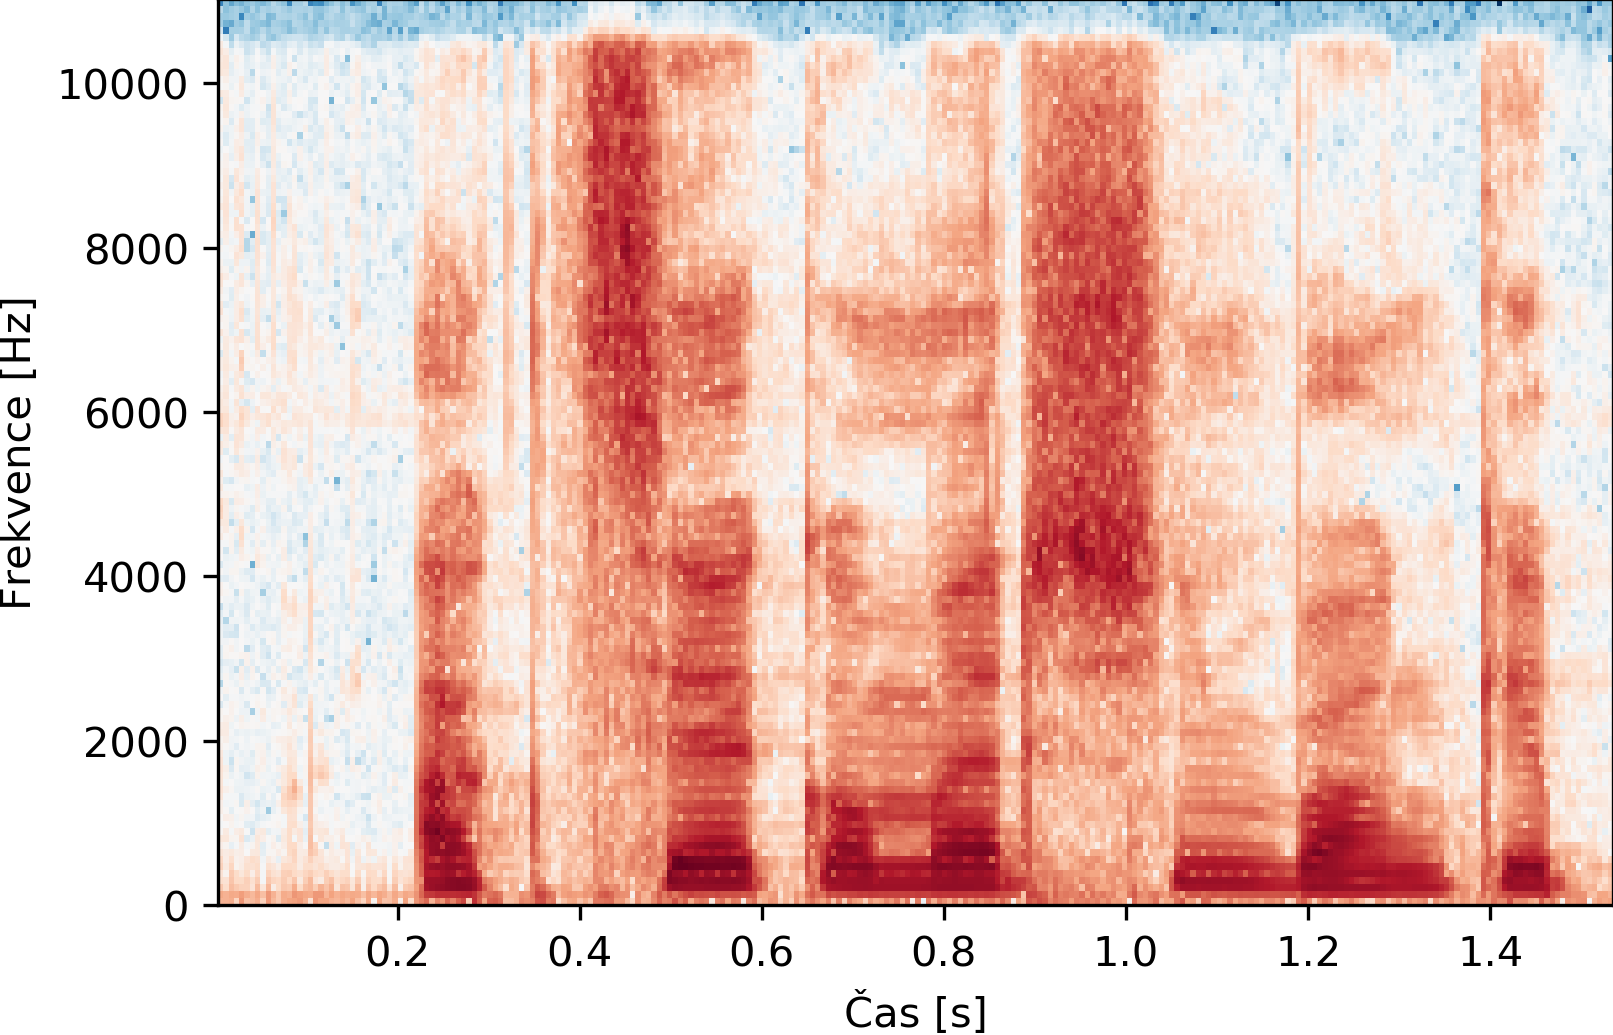
\includegraphics[width=\textwidth]{./ch4-experiments/img/spectrogram0.png}
    \caption{Zdravý řečník}
    \label{fig:experiments:analysis:spectrogram:normal}
  \end{subfigure}
  %
  \begin{subfigure}[b]{0.4\textwidth}
    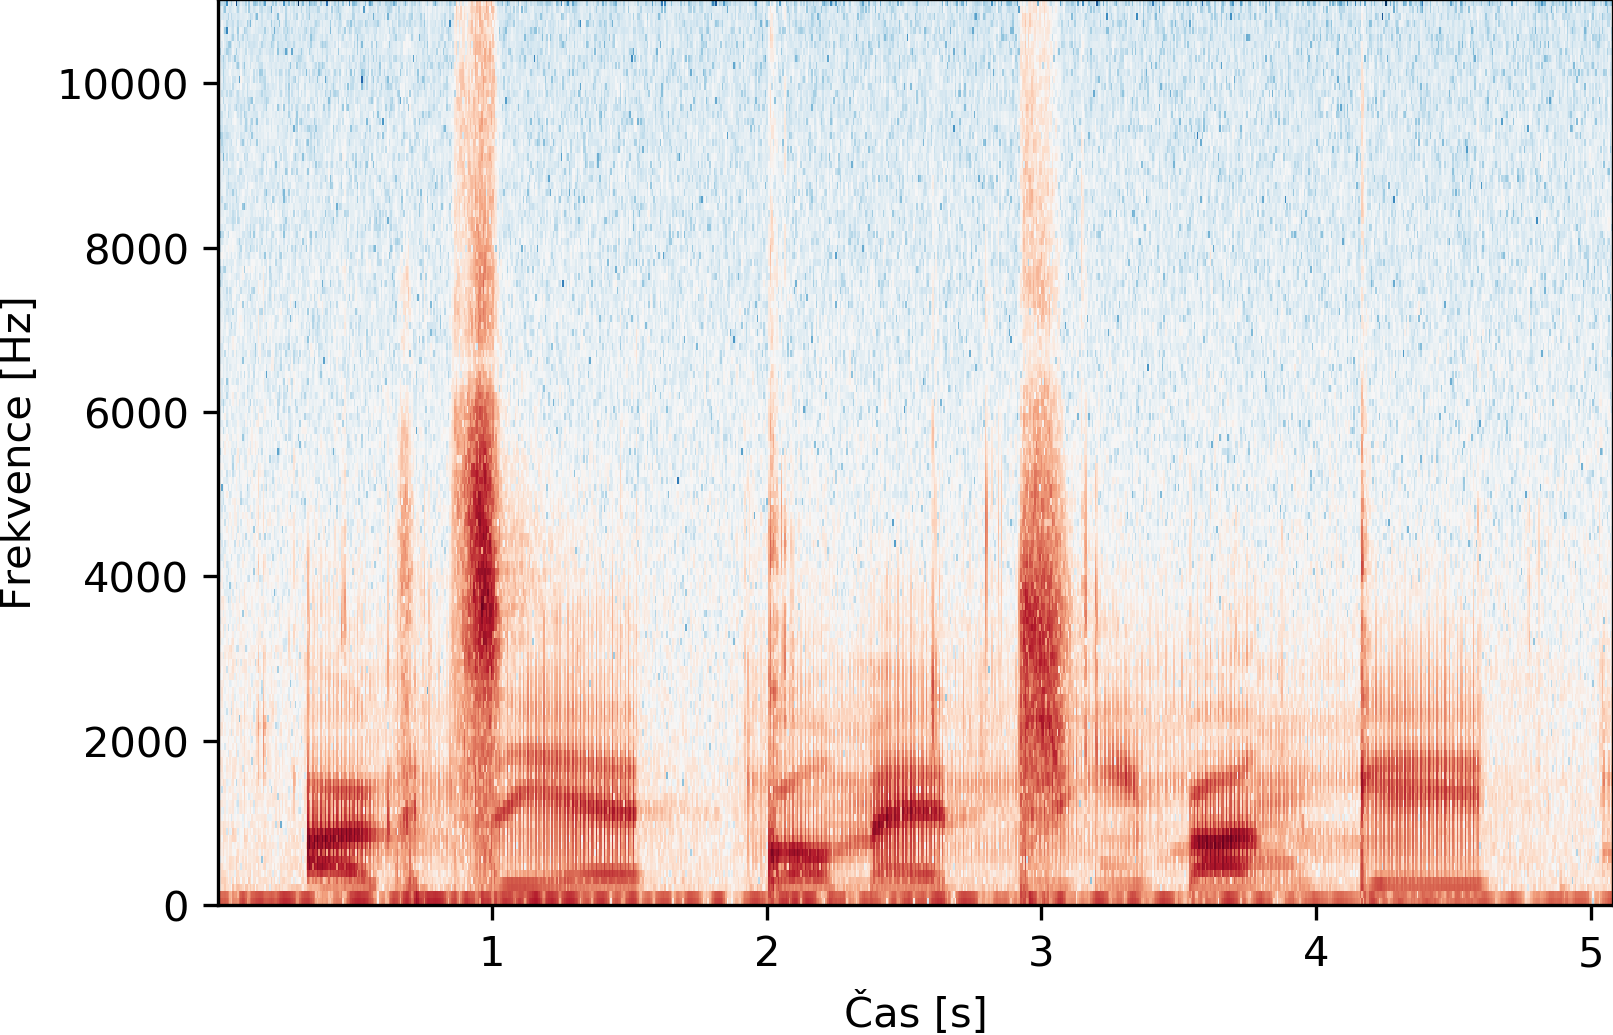
\includegraphics[width=\textwidth]{./ch4-experiments/img/spectrogram1.png}
    \caption{EL řečník}
    \label{fig:experiments:analysis:spectrogram:el}
  \end{subfigure}
  \caption{Spektrogram promluvy \uv{Akcie Komerční banky} dvou řečníků.}
  \label{fig:experiments:analysis:spectrogram}
\end{figure}

test \ref{fig:experiments:analysis:spectrogram} \ref{fig:experiments:analysis:spectrogram:el} \ref{fig:experiments:analysis:spectrogram:normal}

% \begin{figure}[]
%   \centering
%   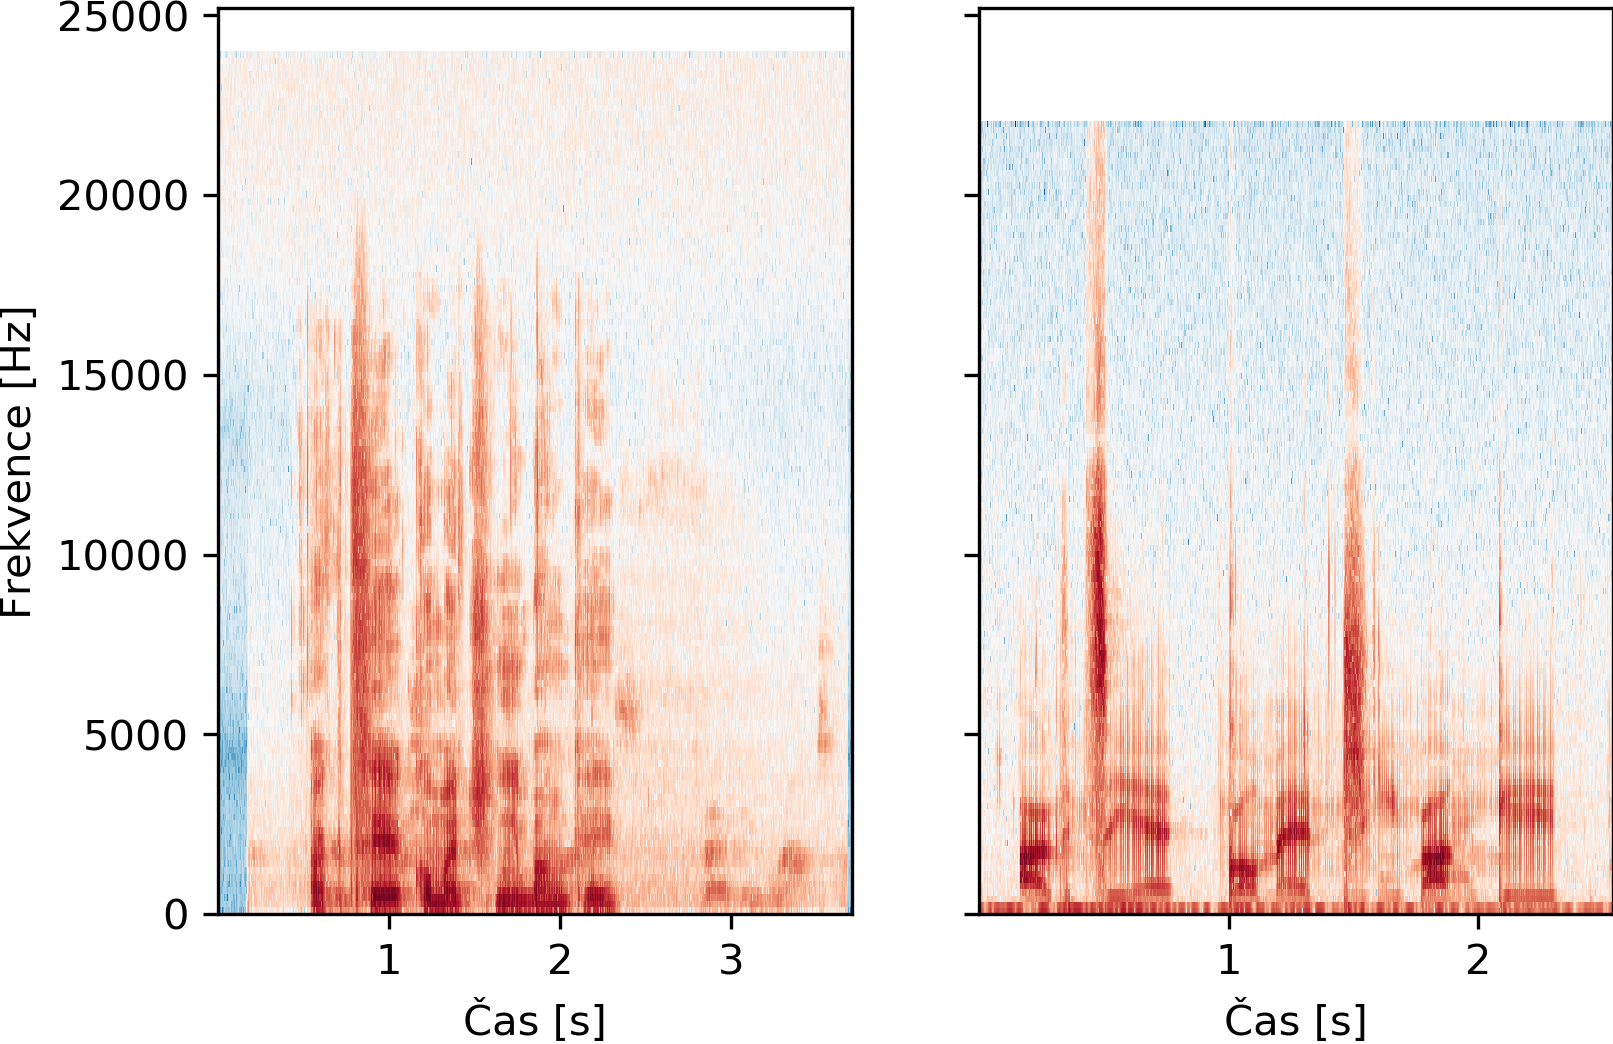
\includegraphics[width=\textwidth]{./ch4-experiments/img/spectrogram_subplot.png}
%   \caption{}
%   \label{}
% \end{figure}

% \csvautotabular{./ch4-experiments/test.csv}

\begin{table}[htpb]
  \centering
  \def\arraystretch{1.5}
  \pgfplotstabletypeset[
    col sep=comma,
    string type,
    columns/model/.style={column name=Model, column type={|c}},
    columns/8k/.style={column name=8 kHz $[\%]$, column type={|r}},
    columns/16k/.style={column name=16 kHz $[\%]$, column type={|r|}},
    every head row/.style={before row={
      \hline
      & \multicolumn{2}{c|}{WER} \\
    },after row=\hline},
    every last row/.style={after row=\hline},
  ]{./ch4-experiments/tabs/01-frequency.csv}
  \caption{Vliv frekvence na kvalitu modelu.}
\end{table}

\begin{itemize}
  \item popis jak byla data získána
  \item informace o datech (frakvenční rozsah, atp.)
  \item prvotní experimenty k určení parametrů modelu
  \item popsat výsledky, výsledky převážně na HTK (HMM + GMM)
\end{itemize}
